\documentclass[12pt]{article}

%%%%%%%%%%%%%%%%%%%%%%%%%%%%%%%%%%%%%%%%%%%%%%%%%%%%%%%%%%%%%%%%%%%%%%%%%%%%%%%%
%                           Package preset for homework
%%%%%%%%%%%%%%%%%%%%%%%%%%%%%%%%%%%%%%%%%%%%%%%%%%%%%%%%%%%%%%%%%%%%%%%%%%%%%%%%
% Miscellaneous
\usepackage[margin=1in]{geometry}
\usepackage[utf8]{inputenc}
\usepackage{indentfirst}
\usepackage{blindtext}
\usepackage{graphicx}
\usepackage{xr-hyper}
\usepackage{hyperref}
\usepackage{enumitem}
\usepackage{color}
\usepackage{float}
% Math
\usepackage{latexsym}
\usepackage{amsfonts}
\usepackage{amssymb}
\usepackage{amsmath}
\usepackage{commath}
\usepackage{amsthm}
\usepackage{bbold}
\usepackage{bm}
% Physics
\usepackage{physics}
\usepackage{siunitx}
% Code typesetting
\usepackage{listings}
% Citation
\usepackage[authoryear]{natbib}
\usepackage{appendix}
\usepackage[capitalize]{cleveref}
% Title & name
\title{Homework}
\author{Tien Vo}
\date{\today}


%%%%%%%%%%%%%%%%%%%%%%%%%%%%%%%%%%%%%%%%%%%%%%%%%%%%%%%%%%%%%%%%%%%%%%%%%%%%%%%%
%                   User-defined commands and environments
%%%%%%%%%%%%%%%%%%%%%%%%%%%%%%%%%%%%%%%%%%%%%%%%%%%%%%%%%%%%%%%%%%%%%%%%%%%%%%%%
%%% Misc
\sisetup{load-configurations=abbreviations}
\newcommand{\due}[1]{\date{Due: #1}}
\newcommand{\hint}{\textit{Hint}}
\let\oldt\t
\renewcommand{\t}[1]{\text{#1}}

%%% Bold sets & abbrv
\newcommand{\N}{\mathbb{N}}
\newcommand{\Z}{\mathbb{Z}}
\newcommand{\R}{\mathbb{R}}
\newcommand{\Q}{\mathbb{Q}}
\let\oldP\P
\renewcommand{\P}{\mathbb{P}}
\newcommand{\LL}{\mathcal{L}}
\newcommand{\FF}{\mathcal{F}}
\newcommand{\HH}{\mathcal{H}}
\newcommand{\NN}{\mathcal{N}}
\newcommand{\ZZ}{\mathcal{Z}}
\newcommand{\RN}[1]{\textup{\uppercase\expandafter{\romannumeral#1}}}
\newcommand{\ua}{\uparrow}
\newcommand{\da}{\downarrow}

%%% Unit vectors
\newcommand{\xhat}{\vb{\hat{x}}}
\newcommand{\yhat}{\vb{\hat{y}}}
\newcommand{\zhat}{\vb{\hat{z}}}
\newcommand{\nhat}{\vb{\hat{n}}}
\newcommand{\rhat}{\vb{\hat{r}}}
\newcommand{\phihat}{\bm{\hat{\phi}}}
\newcommand{\thetahat}{\bm{\hat{\theta}}}

%%% Other math stuff
\providecommand{\units}[1]{\,\ensuremath{\mathrm{#1}}\xspace}
% Set new style for problem
\newtheoremstyle{problemstyle}  % <name>
        {10pt}                   % <space above>
        {10pt}                   % <space below>
        {\normalfont}           % <body font>
        {}                      % <indent amount}
        {\bfseries\itshape}     % <theorem head font>
        {\normalfont\bfseries:} % <punctuation after theorem head>
        {.5em}                  % <space after theorem head>
        {}                      % <theorem head spec (can be left empty, 
                                % meaning `normal')>

% Set problem environment
\theoremstyle{problemstyle}
\newtheorem{problemenv}{Problem}[section]
\newenvironment{problem}[1]{%
  \renewcommand\theproblemenv{#1}%
  \problemenv
}{\endproblemenv}
% Set lemma environment
\newenvironment{lemma}[2][Lemma]{\begin{trivlist}
\item[\hskip \labelsep {\bfseries #1}\hskip \labelsep {\bfseries #2.}]}{\end{trivlist}}
% Set solution environment
\newenvironment{solution}{
    \begin{proof}[Solution]$ $\par\nobreak\ignorespaces
}{\end{proof}}
\numberwithin{equation}{problemenv}

%%% Page format
\setlength{\parindent}{0.5cm}
\setlength{\oddsidemargin}{0in}
\setlength{\textwidth}{6.5in}
\setlength{\textheight}{8.8in}
\setlength{\topmargin}{0in}
\setlength{\headheight}{18pt}

%%% Code environments
\definecolor{dkgreen}{rgb}{0,0.6,0}
\definecolor{gray}{rgb}{0.5,0.5,0.5}
\definecolor{mauve}{rgb}{0.58,0,0.82}
\lstset{frame=tb,
  language=Python,
  aboveskip=3mm,
  belowskip=3mm,
  showstringspaces=false,
  columns=flexible,
  basicstyle={\small\ttfamily},
  numbers=none,
  numberstyle=\tiny\color{gray},
  keywordstyle=\color{blue},
  commentstyle=\color{dkgreen},
  stringstyle=\color{mauve},
  breaklines=true,
  breakatwhitespace=true,
  tabsize=4
}
\lstset{
  language=Mathematica,
  numbers=left,
  numberstyle=\tiny\color{gray},
  numbersep=5pt,
  breaklines=true,
  captionpos={t},
  frame={lines},
  rulecolor=\color{black},
  framerule=0.5pt,
  columns=flexible,
  tabsize=2
}


\title{Homework 11: Phys 7310 (Fall 2021)}

\begin{document}
\maketitle
%%%%%%%%%%%%%%%%%%%%%%%%%%%%%%%%%%%%%%%%%%%%%%%%%%%%%%%%%%%%%%%%%%%%%%%%%%%%%%%
\begin{problem}{11.1}[Magnetic monopoles]
(a) Consider Maxwell's equations with free space permittivity $\epsilon_0$ and
permeability $\mu_0$. Show that when $\rho=\vb{J}=0$, these equations obey a
\textit{duality symmetry} under which
\begin{equation}
    \vb{E}\to c\vb{B}\qquad\text{and}\qquad
    \vb{B}\to-\frac{\vb{E}}{c}
\end{equation}
When $\rho$ and $\vb{J}$ are non-zero, the duality symmetry doesn't exist. Show
that the duality symmetry can be restored by adding magnetic charges with
density $\rho_m$ and current $\vb{J}_m$ to Maxwell's equations in suitable
places, and also including an action of duality on the charges and currents
which you should determine. Thus with magnetic charges added, electrodynamics is
fully symmetric between electric and magnetic phenomena.

(b) Consider a vector potential in spherical coordinates
\begin{equation}\label{p1:A}
    \vb{A}=\frac{g(1-\cos\theta)}{r\sin\theta}\phihat 
\end{equation}
where $g$ is a constant. Show that the associated magnetic field $\vb{B}$ is
the field of a \textit{magnetic monopole}, that is, a Coulomb magnetic field.
What quantity plays the role of ``magnetic charge''?

(c) If there is a magnetic Coulomb field, then the divergence of the magnetic
field is not zero at the origin. However, we expect that any divergence of a
curl of something well-defined is \textit{always} zero. We should therefore ask
what went wrong. What went wrong is that the vector potential above is not
well-defined everywhere. Where besides the origin is the vector potential
$\vb{A}$ singular? Be sure to treat apparently indeterminate quantities
carefully. The locus of singularities is called the \textit{Dirac string}.

If we have a magnetic monopole we can never get rid of the Dirac string, but
gauge transformations can move it around. Define the new vector potential
\begin{equation}\label{p1:Ap}
    \vb{A}'=\frac{g(-1-\cos\theta)}{r\sin\theta}\phihat  
\end{equation}
Find a gauge transformation relating $\vb{A}'$ to $\vb{A}$. Where is the Dirac
string for $\vb{A}'$?

Other gauge transformations can move the string to other locations. Since the
location of the Dirac string is arbitrary and it only shows up in $\vb{A}$,
never in $\vb{B}$, it is not a physical object. (One may think of it
intuitively as like the end of an infinitely thin, infinitely long solenoid,
or an infinitely long chain of dipoles, either way unobservable; see Jackson
figure 6.8). To be well-defined everywhere, we must use more than one vector
potential, such as $\vb{A}$ and $\vb{A}'$ , since each one is singular
somewhere.    

(d) In quantum mechanics, when one performs a gauge transformation on $\Phi$ and
$\vb{A}$ as in Jackson (6.12) and (6.13), one must also perform a gauge
transformation on the wavefunction $\psi(\vb{x},t)$. If the particle has charge
$q$, this gauge transformation is
\begin{equation}
    \psi(\vb{x},t)\to\psi(\vb{x},t)'=e^{iq\Lambda(\vb{x},t)/\hbar}\psi(\vb{x},t) 
\end{equation}
One may show that the Schr\"{o}dinger equation then transforms in a well-defined
way under gauge transformations.

Imagine such a particle of charge $q$ is moving around in the presence of the
magnetic monopole. If we use the two different vector potentials $\vb{A}$ and
$\vb{A}'$, we must use two wave-functions $\psi$ and $\psi'$ for the same
particle. Assuming the wavefunction $\psi$ is well-defined, the wavefunction
$\psi'$ will only be well-defined if
$e^{iq\Lambda/\hbar}(\phi=0)=e^{iq\Lambda/\hbar}(\phi=2\pi)$, since
$\phi=0,2\pi$ represent the same point. What constraint must we place on $q$ and
$g$ to ensure $\psi'$ is well-defined? This constraint is called \textit{Dirac
quantization condition}. If a magnetic monopole exists (none has ever been
observed, but a wide class of so-called grand unified theories predict they
might), what must we conclude about every electric charge in the universe?
\begin{solution}
(a) When $\rho=\vb{J}=0$, Maxwell equations read
\begin{equation}
    \div{\vb{E}}=0,\qquad
    \div{\vb{B}}=0,\qquad
    \curl{\vb{E}}=-\frac{\partial\vb{B}}{\partial t},\qquad
    \curl{\vb{B}}=\frac1{c^2}\frac{\partial\vb{E}}{\partial t}
\end{equation}
Now, let $\vb{E}'=c\vb{B}$, $\vb{B}'=-\vb{E}/c$ and plug into the Maxwell
equations. We get
\begin{align}
    \div{\vb{E}'}&=c\div{\vb{B}}=0\notag\\
    \div{\vb{B}'}&=-\frac1c\div{\vb{E}}=0\notag\\
    \curl{\vb{E}'}&=c\curl{\vb{B}}=\frac1c\frac{\partial\vb{E}}{\partial t}
    =-\frac{\partial\vb{B}'}{\partial t}\notag\\
    \curl{\vb{B}'}&=-\frac1c\curl{\vb{E}}=\frac1c\frac{\partial\vb{B}}{\partial
    t}=\frac1{c^2}\frac{\partial\vb{E}'}{\partial t}
\end{align}
Thus, the Maxwell equations are invariant under this transformation. Now, we
rewrite Maxwell equations with the magnetic charge density $\rho_m$ and current
$\vb{J}_m$
\begin{equation}
    \div{\vb{E}}=\frac{\rho}{\epsilon_0},\qquad
    \div{\vb{B}}=\mu_0\rho_m,\qquad
    \curl{\vb{E}}=-\mu_0\vb{J}_m-\frac{\partial\vb{B}}{\partial t},\qquad
    \curl{\vb{B}}=\mu_0\vb{J}+\frac1{c^2}\frac{\partial\vb{E}}{\partial t}
\end{equation}
Then under the same transformation $\vb{E}'=c\vb{B},\vb{B}'=-\vb{E}'/c$, they
become
\begin{align}
    \div{\vb{E}'}&=c\div{\vb{B}}=\frac{\rho_m/c}{\epsilon_0}\notag\\
    \div{\vb{B}'}&=-\frac1c\div{\vb{E}}=\mu_0\qty(-c\rho)\notag\\
    \curl{\vb{E}'}&=c\curl{\vb{B}}=c\qty(\mu_0\vb{J}+\frac1{c^2}\frac{\partial\vb{E}}{\partial
    t})=-\mu_0\qty(-c\vb{J})-\frac{\partial\vb{B}'}{\partial t}\notag\\
        \curl{\vb{B}'}&=-\frac1c\curl{\vb{E}}=\mu_0\frac{\vb{J}_m}{c}+\frac1{c^2}\frac{\partial\vb{E}'}{\partial
        t}
\end{align}
Thus, this transformation turns
$\rho,\rho_m,\vb{J},\vb{J}_m\mapsto\rho',\rho_m',\vb{J}',\vb{J}_m'$ where
\begin{equation}
    \rho_m=c\rho',\qquad
    \rho=-\frac1c\rho_m',\qquad
    \vb{J}=-\frac1c\vb{J}_m',\qquad
    \vb{J}_m=c\vb{J}'
\end{equation}
Formally, Maxwell equations are still invariant, so the \textit{duality 
symmetry} is restored if we add $\rho_m,\vb{J}_m$ as above.

(b) The corresponding magnetic field $\vb{B}$ is
\begin{equation}
    \vb{B}=\curl{\vb{A}}
    =\frac1{r\sin\theta}\frac{\partial}{\partial\theta}\qty(A\sin\theta)\rhat
    -\frac1r\frac{\partial}{\partial r}\qty(rA)\thetahat
    =\frac{g}{r^2}\rhat
\end{equation}
Thus, this is a Coulomb field (radial and the magnitude follows an inverse
square law). The constant $g$ here plays the role of magnetic charge.

(c) Given $\vb{A},\vb{A}'$ in \eqref{p1:A} and \eqref{p1:Ap}, we plot the polar
angle dependence in the figure below.
\begin{center}
    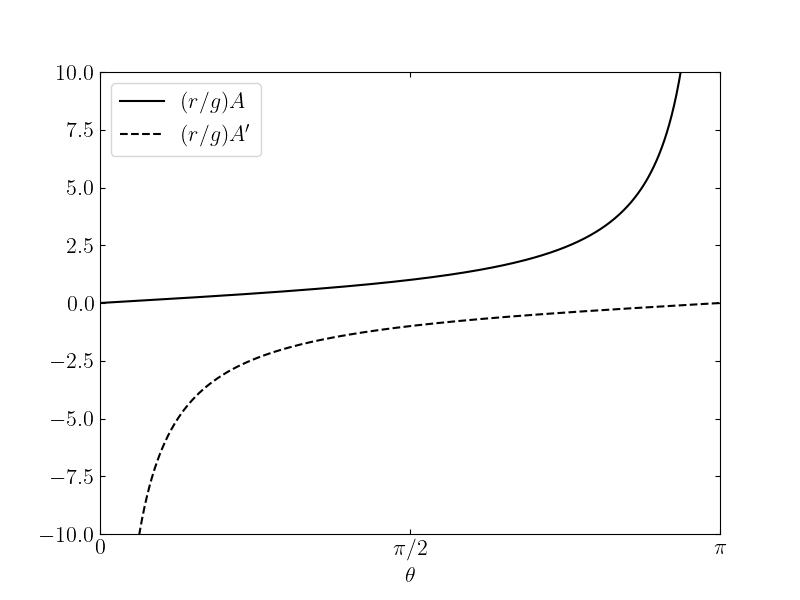
\includegraphics[width=0.7\textwidth]{p1.png}
\end{center}
Then $\vb{A}$ has a pole at $\theta=\pi$, beside at the origin and $\vb{A}'$ has
a pole at $\theta=0$. Now, we want to find $\Lambda$ such that
$\vb{A}'=\vb{A}+\grad\Lambda$. Thus, it follows that
\begin{equation}
    \frac{1}{r\sin\theta}\frac{\partial\Lambda}{\partial\phi}=-\frac{2g}{r\sin\theta}\Rightarrow\Lambda=-2g\phi 
\end{equation}

(d) For $\psi'$ to be well-defined, it must be that
\begin{equation}
    1=\exp\qty(-\frac{4\pi iqg}{\hbar})=\cos\qty(\frac{4\pi
    qg}{\hbar})-i\sin\qty(\frac{4\pi qg}{\hbar})
\end{equation}
Thus, we must require $4\pi qg/\hbar=n2\pi$ for $n\in\Z$, or
\begin{equation}
    \frac{qg}{\hbar}=\frac{n}{2} 
\end{equation}
If a magnetic monopole exists, then the electric charge must be quantized.
\end{solution}
\end{problem}
%%%%%%%%%%%%%%%%%%%%%%%%%%%%%%%%%%%%%%%%%%%%%%%%%%%%%%%%%%%%%%%%%%%%%%%%%%%%%%%
%%%%%%%%%%%%%%%%%%%%%%%%%%%%%%%%%%%%%%%%%%%%%%%%%%%%%%%%%%%%%%%%%%%%%%%%%%%%%%%
\begin{problem}{11.2}[Polarizations of EM radiation]
Consider an electromagnetic wave in free space, where $\epsilon=\epsilon_0$ and
$\mu=\mu_0$, and there are no charges or currents nearby. The wave has frequency
$\omega$. Let the direction of travel of the wave be $\zhat$, so that Jackson's
$\hat\epsilon_1$ and $\hat\epsilon_2$ are just $\xhat$ and $\yhat$.

(a) Assuming the (complex) electric field is given by Jackson (7.19) with
$E_1=E_2=E$, find the \textit{real} electric field. Determine its amplitude
$E_0$ (this might not be the same as $E$!) and a unit polarization vector
characterizing its direction. Find the real form of $\vb{B}$ as well, including
magnitude and direction. Calculate the time-averaged energy density in two ways,
one by finding the (real, time-dependent) energy density using the real fields
(Jackson 6.106 in free space) and then time-averaging, and the other by using
the complex time-averaged formula (the equation above Jackson (7.14)) and show
your result agrees with Jackson (7.14) with $\epsilon\to\epsilon_0$. Is the
direction of polarization changing with time? Is this wave linearly polarized,
circularly polarized, or neither?

(b) Do all the same things and answer all the same questions for the case
$E_1=E,E_2=iE$.
\begin{solution}
(a) First, given $\vb{k}=k\zhat$, we write the complex electric and magnetic
fields
\begin{equation}
    \vb{E}=E(\xhat+\yhat)e^{i(kz-\omega t)},\qquad
    \vb{B}=\frac1\omega\vb{k}\times\vb{E}=\frac{kE}{\omega}\qty(\yhat-\xhat)e^{i(kz-\omega
    t)}
\end{equation}
The real electric and magnetic fields are thus
\begin{equation}
    \vb{E}_R=E\qty(\xhat+\yhat)\cos\qty(kz-\omega t),\qquad
    \vb{B}_R=\frac{kE}{\omega}\qty(\yhat-\xhat)\cos\qty(kz-\omega t)
\end{equation}
The corresponding amplitudes are $E_0=\sqrt{2}E$ and $B_0=kE_0/\omega$. The unit
polarization vector of the electric field is $\bm\epsilon=(\xhat+\yhat)/\sqrt2$.
The energy density is, using (6.106, Jackson)
\begin{equation}
    u=\frac12\qty(\epsilon_0E_R^2+\frac{B_R^2}{\mu_0})=\epsilon_0E^2\qty(1+n^2)\cos^2(kz-\omega
    t)\Rightarrow\expval{u}=\frac12\epsilon_0E^2(1+n^2) 
\end{equation}
where $n=ck/\omega$ is the index of refraction. Now, the energy density using
(7.14, Jackson) is
\begin{equation}
    \expval{u}=\frac14\qty(2\epsilon_0E^2+\frac{2k^2E^2}{\omega^2\mu_0}) 
    =\frac12\epsilon_0E^2\qty(1+n^2)
\end{equation}
These results agree. The polarization $\bm\epsilon$ does not change in time, and
the wave is linearly polarized.

(b) The complex fields are
\begin{equation}
    \vb{E}=E(\xhat+i\yhat)e^{i(kz-\omega t)},\qquad
    \vb{B}=\frac{kE}{\omega}\qty(\yhat-i\xhat)e^{i(kz-\omega t)}
\end{equation}
Then the real fields are
\begin{equation}
    \vb{E}_R=E\qty[\cos(kz-\omega t)\xhat-\sin(kz-\omega t)\yhat],\qquad
    \vb{B}_R=\frac{kE}{\omega}\qty[\sin(kz-\omega t)\xhat+\cos(kz-\omega t)\yhat]
\end{equation}
The amplitudes are still $E_0=\sqrt2E$ and $B_0=kE_0/\omega$. The polarization
of the electric field is $\bm\epsilon=(\xhat+i\yhat)/\sqrt2$. In this case, it
rotates clockwise in a plane perpendicular to $\vb{k}$ in time. Since the
amplitude is the same, the energy density using (7.14, Jackson) should give the
same result. Now, from the real fields,
\begin{equation}
    u=\frac12\qty(\epsilon_0E^2+\frac{k^2E^2}{\omega^2\mu_0})
    =\frac12\epsilon_0E^2(1+n^2)\Rightarrow\expval{u}=\frac12\epsilon_0E^2(1+n^2)
\end{equation}
\end{solution}
\end{problem}
%%%%%%%%%%%%%%%%%%%%%%%%%%%%%%%%%%%%%%%%%%%%%%%%%%%%%%%%%%%%%%%%%%%%%%%%%%%%%%%
%%%%%%%%%%%%%%%%%%%%%%%%%%%%%%%%%%%%%%%%%%%%%%%%%%%%%%%%%%%%%%%%%%%%%%%%%%%%%%%
\begin{problem}{11.3}[Reflection and transmission at a layered interface]
A plane wave is incident on a layered interface as shown in the figure. The
indices of refraction of the three nonpermeable media are $n_1,n_2,n_3$. The
thickness of the intermediate layer is $d$. Each of the other media is
semi-infinite.

(a) Calculate the transmission and reflection coefficients (ratios of
transmitted and reflected Poynting's flux to the incident flux), and sketch
their behavior as a function of frequency for
$n_1=1,n_2=2,n_3=3;n_1=3,n_2=2,n_3=1;$ and $n_1=2,n_2=4,n_3=1$.

(b) The medium $n_1$ is part of an optical system (e.g., a lens); medium $n_3$
is air ($n_3=1$). It is desired to put an optical coating (medium $n_2$) on the
surface so that there is no reflected wave for a frequency $\omega_0$. What
thickness $d$ and index of refraction $n_2$ are necessary?
\begin{solution}
(a) First, in medium 1, the fields are a superposition of an incident and
reflected wave
\begin{align}
    \vb{E}_i&=E_ie^{i(k_1z-\omega t)}\xhat &
    \vb{B}_i&=\frac{E_i}{v_1}e^{i(k_1z-\omega t)}\yhat\notag\\
    \vb{E}_R&=E_Re^{i(-k_1z-\omega t)}\xhat &
    \vb{B}_R&=-\frac{E_R}{v_1}e^{i(-k_1z-\omega t)}\yhat\notag\\
\end{align}
where $v_1=1/\sqrt{\epsilon_1\mu_1}=c/n_1=\omega/k_1$. In medium 2, there are
also backward and forward propagating waves
\begin{align}
    \vb{E}_+&=E_+e^{i(k_2z-\omega t)}\xhat &
    \vb{B}_+&=\frac{E_+}{v_2}e^{i(k_2z-\omega t)}\yhat\notag\\
    \vb{E}_-&=E_-e^{i(-k_2z-\omega t)}\xhat &
    \vb{B}_-&=-\frac{E_-}{v_2}e^{i(-k_2z-\omega t)}\yhat\notag\\
\end{align}
And in medium 3, there is only a transmitted wave since there is no surface to
reflect off of
\begin{align}
    \vb{E}_T&=E_Te^{i(k_3z-\omega t)}\xhat &
    \vb{B}_T&=\frac{E_T}{v_3}e^{i(k_3z-\omega t)}\yhat
\end{align}
We then apply the boundary conditions (7.37) for $z=0$ and $z=d$ (assuming the
1--2 interface is at $z=0$ and 2--3 interface is at $z=d$) of the parallel
fields
\begin{subequations}
    \begin{align}
        E_i+E_R&=E_++E_-\label{p3a:1}\\
        E_+e^{ik_2d}+E_-e^{-ik_2d}&=E_Te^{ik_3d}\label{p3a:2}\\
        E_i-E_R&=\frac{v_1}{v_2}\qty(E_+-E_-)\label{p3a:3}\\
        E_+e^{ik_2d}-E_-e^{-ik_2d}&=\frac{v_2}{v_3}E_Te^{ik_3d}\label{p3a:4}
    \end{align} 
\end{subequations}
where we have also let $\mu_1=\mu_2=\mu_3$. Since $v_j=c/n_j$, it is also 
possible to write $v_1/v_2=n_2/n_1$ and $v_2/v_3=n_3/n_2$. Solving this system
with Mathematica yields
\begin{equation}
    E_+=\frac12\qty(1+\frac{n_3}{n_2})e^{i(k_3-k_2)d}E_T\qquad\text{and}\qquad
    E_-=\frac12\qty(1-\frac{n_3}{n_2})e^{i(k_3+k_2)d}E_T
\end{equation}
Adding \eqref{p3a:1} and \eqref{p3a:3}, we can write
\begin{align}
    2E_i
    &=\qty(1+\frac{n_2}{n_1})E_++\qty(1-\frac{n_2}{n_1})E_-\notag\\
    &=\frac12\qty[\qty(1+\frac{n_2}{n_1})\qty(1+\frac{n_3}{n_2})e^{i(k_3-k_2)d}+\qty(1-\frac{n_2}{n_1})\qty(1-\frac{n_3}{n_2})e^{i(k_3+k_2)d}]E_T
\end{align}
Then it follows that
\begin{equation}
    \frac{E_T^2}{E_i^2}=4\qty[\qty(1+\frac{n_3}{n_1})^2\cos^2x+\qty(\frac{n_2}{n_1}+\frac{n_3}{n_2})^2\sin^2x]^{-1} 
\end{equation}
where $x=n_2d\omega/c$. From (7.13, Jackson), the transmission coefficient is
\begin{align}
    T&=\frac{S_T^2}{S_i^2}\notag\\
     &=\frac{\sqrt{\epsilon_3/\mu_3}E_T^2}{\sqrt{\epsilon_1/\mu_1}E_i^2}\notag\\
     &=\frac{n_3}{n_1}\frac{E_T^2}{E_i^2}\notag\\
     &=4\frac{n_3}{n_1}\qty[\qty(1+\frac{n_3}{n_1})^2+\qty(\frac{n_2^2}{n_1^2}+\frac{n_3^2}{n_2^2}-\frac{n_3^2}{n_1^2}-1)\sin^2x]^{-1}\notag\\
     &=\frac{4n_1n_2^2n_3}{n_2^2(n_1+n_3)^2+[n_2^2(n_2^2-n_3^2)+n_1^2(n_3^2-n_2^2)]\sin^2x}
\end{align}
Then it follows that the reflection coefficient is
\begin{equation}\label{p3:b}
    R=1-T=1-\frac{4n_1n_2^2n_3}{n_2^2(n_1+n_3)^2+[n_2^2(n_2^2-n_3^2)+n_1^2(n_3^2-n_2^2)]\sin^2x}
\end{equation}

In the figure below, we show $T$ (solid lines) and $R$ (dotted lines) in three
cases: $(n_1,n_2,n_3)\in\qty{(1,2,3),(3,2,1),(2,4,1)}$. The first two cases
(black and red) lay on top of each other.
\begin{center}
    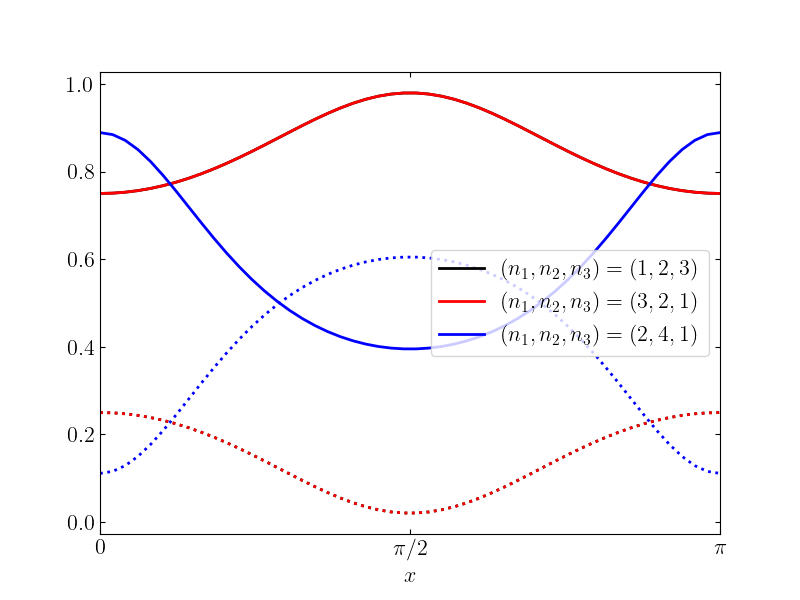
\includegraphics[width=0.7\textwidth]{p3.png} 
\end{center}

(b) Given $n_3=1$, from \eqref{p3:b}, $R=0$ when
\begin{equation}
    n_2^2(1-n_1)^2+(n_2^2-1)(n_2^2-n_1^2)\sin^2x=0 
    \qquad\text{or}\qquad
    \sin(x)=\frac{n_2(n_1-1)}{\sqrt{(n_2^2-1)(n_1^2-n_2^2)}}
\end{equation}
This requires that $n_1>n_2$ and the thickness is determined by
\begin{equation}
    d=\frac{c\omega_0}{n_2}\sin^{-1}\qty[\frac{n_2(1-n_1)}{\sqrt{(n_2^2-1)(n_1^2-n_2^2)}}] 
\end{equation}
\end{solution}
\end{problem}
%%%%%%%%%%%%%%%%%%%%%%%%%%%%%%%%%%%%%%%%%%%%%%%%%%%%%%%%%%%%%%%%%%%%%%%%%%%%%%%
\end{document}
